\section{Задание}

Изучить и реализовать генератор псевдослучайных чисел программным и табличным методом.
Разрядность чисел должна быть равна 1, 2, 3.
Сравнить методы по определенному критерию и сделать выводы.

\section{Теоритическая часть}

\subsection{Программный генератор}

Программный генератор формирует псевдослучайные числа. Каждое последующее число в такой последовательности зависит от предыдущего.
Сгенерированные числа статистически случайны, несмотря на то, что это полностью детерминированный и повторяемый процесс.

\subsubsection{Линейный конгруэнтный метод}
Генератор определяется рекуррентным соотношением:
\begin{equation*}
    X_{n+1} = (a X_n + c) \ mod \ m
\end{equation*}
где:
\hspace*{.7cm} $m > 0$, модуль \\
\hspace*{1.5cm} $0 <= a <= m$, множитель \\
\hspace*{1.5cm} $0 <= c  <= m$, приращение \\
\hspace*{1.5cm} $0 <= X_0  <= m$, начальное число


\subsection{Табличный генератор}

Табличный генератор использует таблицу проверенных некоррелированных цифр в качестве источника случайных чисел.

\subsection{Критерий равномерности}

Пусть имеется последовательность целых чисел $X_n$, $0 <= X_i < d$.

При оценке равномерности для каждого $r$ ($0 <= r < d$) подсчитывается количество случаев, когда элемент последовательности $X_i=r$.

После этого применяется критерий $\chi^2$, в котором вычисляется статистика: 

\begin{equation*}
	\chi^2 = \sum_{i = 0}^{k - 1} \frac{(x_i - m_i)^2}{m_i}
    \quad \sim \quad \chi^2(k-1)
\end{equation*}

Где $m_i = np_i = n/d$

Рассчитать значение $p$ для уровня погрешность $\alpha = 0.05$ допускать $0.05 < p < 0.95$.

\pagebreak
\section{Результаты}

\begin{figure}[h!]
    \centering
    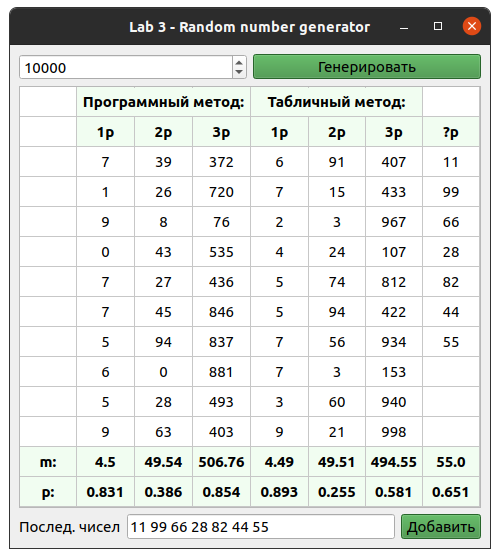
\includegraphics[width=0.58\textwidth]{3/eg1}
    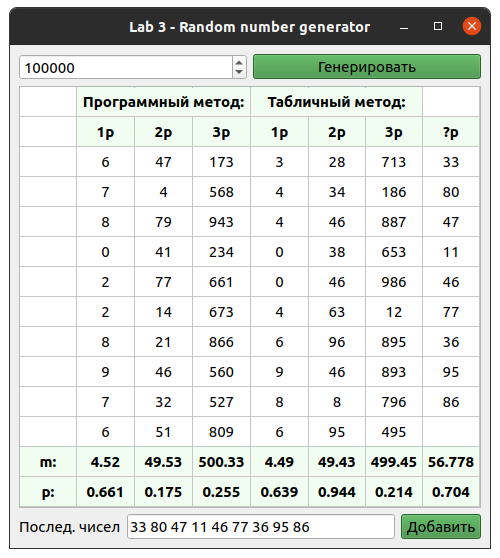
\includegraphics[width=0.58\textwidth]{3/eg2}
\end{figure}

При уровня погрешность $\alpha = 0.05$, $0.05 < p < 0.95$ в большинстве случаев.
Чем больше количество генерируемых случайных чисел, тем равномернее они распределены.
Но для большого количества чисел какая-то закономерность повторяется.

\pagebreak
\section{Листинг кода}

\lstinputlisting[
    language=Python,
    caption=рограммная реализация генерации псевдослучайных чисел программным и табличным методом
]{../3/rand.py}
